\documentclass[default]{beamer}
\setbeamertemplate{navigation symbols}{}

\usetheme{CambridgeUS}
%\useoutertheme{infolines}
\usecolortheme{beaver}

\usepackage[utf8]{inputenc}					% Выбор языка и кодировки
\usepackage[english, russian]{babel}	% Языки: русский, английский
\usepackage{csquotes}
\usepackage{tikz}
\usetikzlibrary{arrows,shapes,calc}
\usepackage{animate}
\usepackage{fp}
\usepackage{media9}
\usepackage{textpos}

\usepackage[
	language=auto,
	autolang=other,
	backend=biber,
	style=authortitle,
	sorting=ydnt,
	maxbibnames=5
]{biblatex}
\addbibresource{panov_causal.bib}
				
\DeclareSourcemap{
	\maps[datatype=bibtex, overwrite]{
		\map{
			\step[fieldset=langid, fieldvalue=english]
			\step[fieldset=doi, null]
			\step[fieldset=issn, null]
			\step[fieldset=isbn, null]
			\step[fieldset=url, null]
			\step[fieldsource=language, fieldset=langid, origfieldval]
		}
	}
}
\DeclareBibliographyDriver{std}{%
	\usebibmacro{bibindex}%
	\usebibmacro{begentry}%
	\usebibmacro{author/editor+others/translator+others}%
	\setunit{\labelnamepunct}\newblock
	\usebibmacro{title}%
	\newunit\newblock
	\usebibmacro{maintitle+booktitle}
	\newunit\newblock
	\usebibmacro{journal}%
	\newunit\newblock
	\usebibmacro{date}%
	\newunit\newblock
	\usebibmacro{finentry}
}
\DeclareBibliographyAlias{article}{std}
\DeclareBibliographyAlias{book}{std}
\DeclareBibliographyAlias{inproceedings}{std}
\DeclareBibliographyAlias{incollection}{std}

\graphicspath{{../../images/}} 			% Пути к изображениям

\makeatletter
\setbeamertemplate{footline}
{
	\leavevmode%
	\hbox{%
		\begin{beamercolorbox}[wd=.333333\paperwidth,ht=2.25ex,dp=1ex,center]{author
				in head/foot}%
			\usebeamerfont{author in
				head/foot}\insertshortauthor~~\beamer@ifempty{\insertshortinstitute}{}{(\insertshortinstitute)}
		\end{beamercolorbox}%
		\begin{beamercolorbox}[wd=.333333\paperwidth,ht=2.25ex,dp=1ex,center]{title in
				head/foot}%
			\usebeamerfont{title in head/foot}\insertshorttitle
		\end{beamercolorbox}%
		\begin{beamercolorbox}[wd=.333333\paperwidth,ht=2.25ex,dp=1ex,right]{date in
				head/foot}%
			\usebeamerfont{date in head/foot}\insertshortdate{}\hspace*{1em}
			\insertframenumber{}\hspace*{2ex} 
		\end{beamercolorbox}
	}%
	\vskip0pt%
}

\addtobeamertemplate{frametitle}{}{
	\begin{textblock*}{100mm}(\textwidth-35pt,-20pt)
		
\includegraphics[width=1.5cm]{misc/logos/frccsc.png}
	\end{textblock*}
}

\newcommand{\predmatr}[3]{
	\node[ell, rectangle, minimum height = 15, minimum width = 7.5]  at (#1 pt,#2 pt) {}; 
	\node[ellf, rectangle, minimum height = 15, minimum width = 7.5] at (#1+7.5 pt,#2 pt) {};
	\node[minimum height = 15, minimum width = 15] (#3) at (#1+3.3pt,#2 pt) {};
	\draw[ell] (#1+7.5 pt,#2+7.5 pt) -- (#1 +7.5 pt,#2-7.5 pt);
}
\renewcommand*{\bibfont}{\tiny}
\setlength\bibitemsep{-5pt}

\begin{document}
	
	\title[Каузальные связи]{Взаимодействие логических и статистических методов анализа психологических данных}
	\author[Панов]{Александр Игоревич Панов}
	\institute[ФИЦ ИУ РАН]{Отдел <<Интеллектуальные динамические системы и когнитивные исследования>>\\Институт системного анализа\\ Федеральный исследовательский центр <<Информатика и управление>>\\Российской академии наук}
	\date[21 марта]{21 марта 2018\\Семинар <<Анализ больших данных в информатике, управлении и психологии>>} 
	
	\begin{frame}
		\titlepage
		\centering
		\includegraphics[width=100pt]{misc/logos/ras.png} \hspace{10pt}
		
\includegraphics[width=80pt]{misc/logos/frccsc.png} \hspace{10pt}
		
\includegraphics[width=20pt]{misc/logos/hse.png}
	\end{frame}

	\begin{frame}
		\frametitle{Корреляционные и причинно-следственные связи}
		\onslide<1->{
			Основа статистических методов анализа данных (факторного, регрессионного и др.) "--- \textbf{корреляционная связь}.
			\par\bigskip
			Корреляция между двумя признаками $A$ и $B$ в наборе данных $X$ "--- не есть каузальная зависимость между признаком $A$ и $B$.
			\par\bigskip
			Классический пример трех признаков: $A$, $B$ $C$. Пусть $A\rightarrow B$, $A\rightarrow C$, тогда при уменьшении или увеличении проявления признака $A$ будет в меньшей или большей степени соответственно проявляться и признаки $B$ и $C$, т.е. $B$ и $C$ будут изменяться согласованно. 
			\par\bigskip
		}
		\onslide<2->{
			\textbf{Между ними будет определен высокий уровень корреляции, что на самом деле не отражает реально имеющихся причинно-следственных связей.}
		}
	\end{frame}
	
	\begin{frame}
		\frametitle{Логические методы}
		\onslide<1->{
			Интеллектуальный анализ данных $\rightarrow$ логические методы анализа "--- моделирование индуктивных и дедуктивных рассуждений, рассуждений по аналогии.
			\par\bigskip
			Интеллектуальные методы позволяют смоделировать процесс принятия решений специалистом в данной предметной области.
			\par\bigskip
			ДСМ-метод "--- метод порождения гипотез о наличии причинно-следственных связей.
			\par\bigskip
		}
		\onslide<3->{
			\textbf{Существенные преимущества}: интерпретируемость и работа в сложном каузальном пространстве со многими классами объектов.
			\par\bigskip
		}
		\onslide<3->{
			\textbf{Существенные недостатки}: комбинаторная сложность (низкая эффективность) и проверка гипотез (высокая доля ложных гипотез).
		}
	\end{frame}
	
	\begin{frame}
		\frametitle{Метод AQJSM}
		\textbf{Основная идея метода}: проверять логические гипотезы статистическими методами.
		\begin{enumerate}
			\item Построение логического описания объектов различных классов.
			\item Формирование базы фактов вида Объекты $times$ Свойства.
			\item Применение первого этапа ДСМ-метода для выдвижения гипотез о наличии причинно-следственных связей.
			\item Фальсификация гипотез путем структурного моделирования.
			\item Отбор прошедших предыдущий этап гипотез.
		\end{enumerate}
	\end{frame}
	
	\begin{frame}
		\frametitle{Формальная постановка}
		\textbf{Дано:}
		\begin{itemize}
			\item Множество $X=\{x_i\}$ "--- множество из $m$ объектов (испытуемых).
			\item Отображение $f_i: X\rightarrow D_j$ "--- признаки объекта, $D=\{d_k^j\}$ "--- шкалы методик и опросников.
			\item $F=\|f_j(x_i)\|_{m\times n}$ "--- матрица объекты-признаки.
			\item $C=\{c_l\}$ "--- множество классов, на которые были разбиты объекты.
			\par\bigskip
		\end{itemize}
		\par\bigskip
		\textbf{Предобработка:}
		\begin{itemize}
			\item Дискретизация интервальных признаков: $(d_1^j,d^j_k)=w_1\cup w_2\cup w_3$.
			\item Переход к свойствам объектов $h^i_k=x_i\in w_k$.
			\item Удаление дублирующих строчек матрицы объекты-свойства $\|f_j(x_i)\|_{m\times n}$.
		\end{itemize}
		\par\bigskip
		AQ-обучение:
		\begin{itemize}
			\item Для каждого класса $c_t$ строим набор AQ-правил вида $R_{ij}\Cap_j\left(d^j=\Cup_q w_q\right)$.
			\item .
		\end{itemize}
	\end{frame}

	\begin{frame}
		\frametitle{Формальная постановка}
		{\scriptsize
		AQ-обучение:
		\begin{itemize}
			\item Для каждого класса $c_t$ выбираем затравочный объект и строим базу правила вида $R_i=\{d_i^1=w_{i_1},\dots, d_i^j=w_{i_j}\}$.
			\item Перебираем примеры класс итерационного обобщая правило, получаем набор AQ-правил вида 
			\[R_{ij}=\bigcap_j\left(d^j=\bigcup_q w_q\right).\]
		\end{itemize}
		\par\bigskip
		Этап ДСМ:
		\begin{itemize}
			\item Составление базы фактов ДСМ-метода "--- битовая матрица $B_{m\times3n}$.
			\item Сокращение пространства поиска "--- удаление противоречивых примеров.
			\item Использование гипотез для выявления каузальных связей:
			\begin{itemize}
				\item \textit{Гипотеза сходства}. 
				\item \textit{Гипотеза различия}. 
				\item \textit{Гипотеза абдукции}. 
			\end{itemize}
			\item Получаем множество гипотез вида:
			\[H(h_g, c_l)=\bigcap_{j\not = g}\left( d^j=\bigcup_q w_q\right).\]
		\end{itemize}
		}
	\end{frame}
	
	\begin{frame}
		\frametitle{Этап AQ обучения}
		
		\centering
		\includegraphics[width=0.6\textwidth]{AQProcess.jpeg}
	\end{frame}

	\begin{frame}
		\frametitle{Этап ДСМ анализа}
		
		\centering
		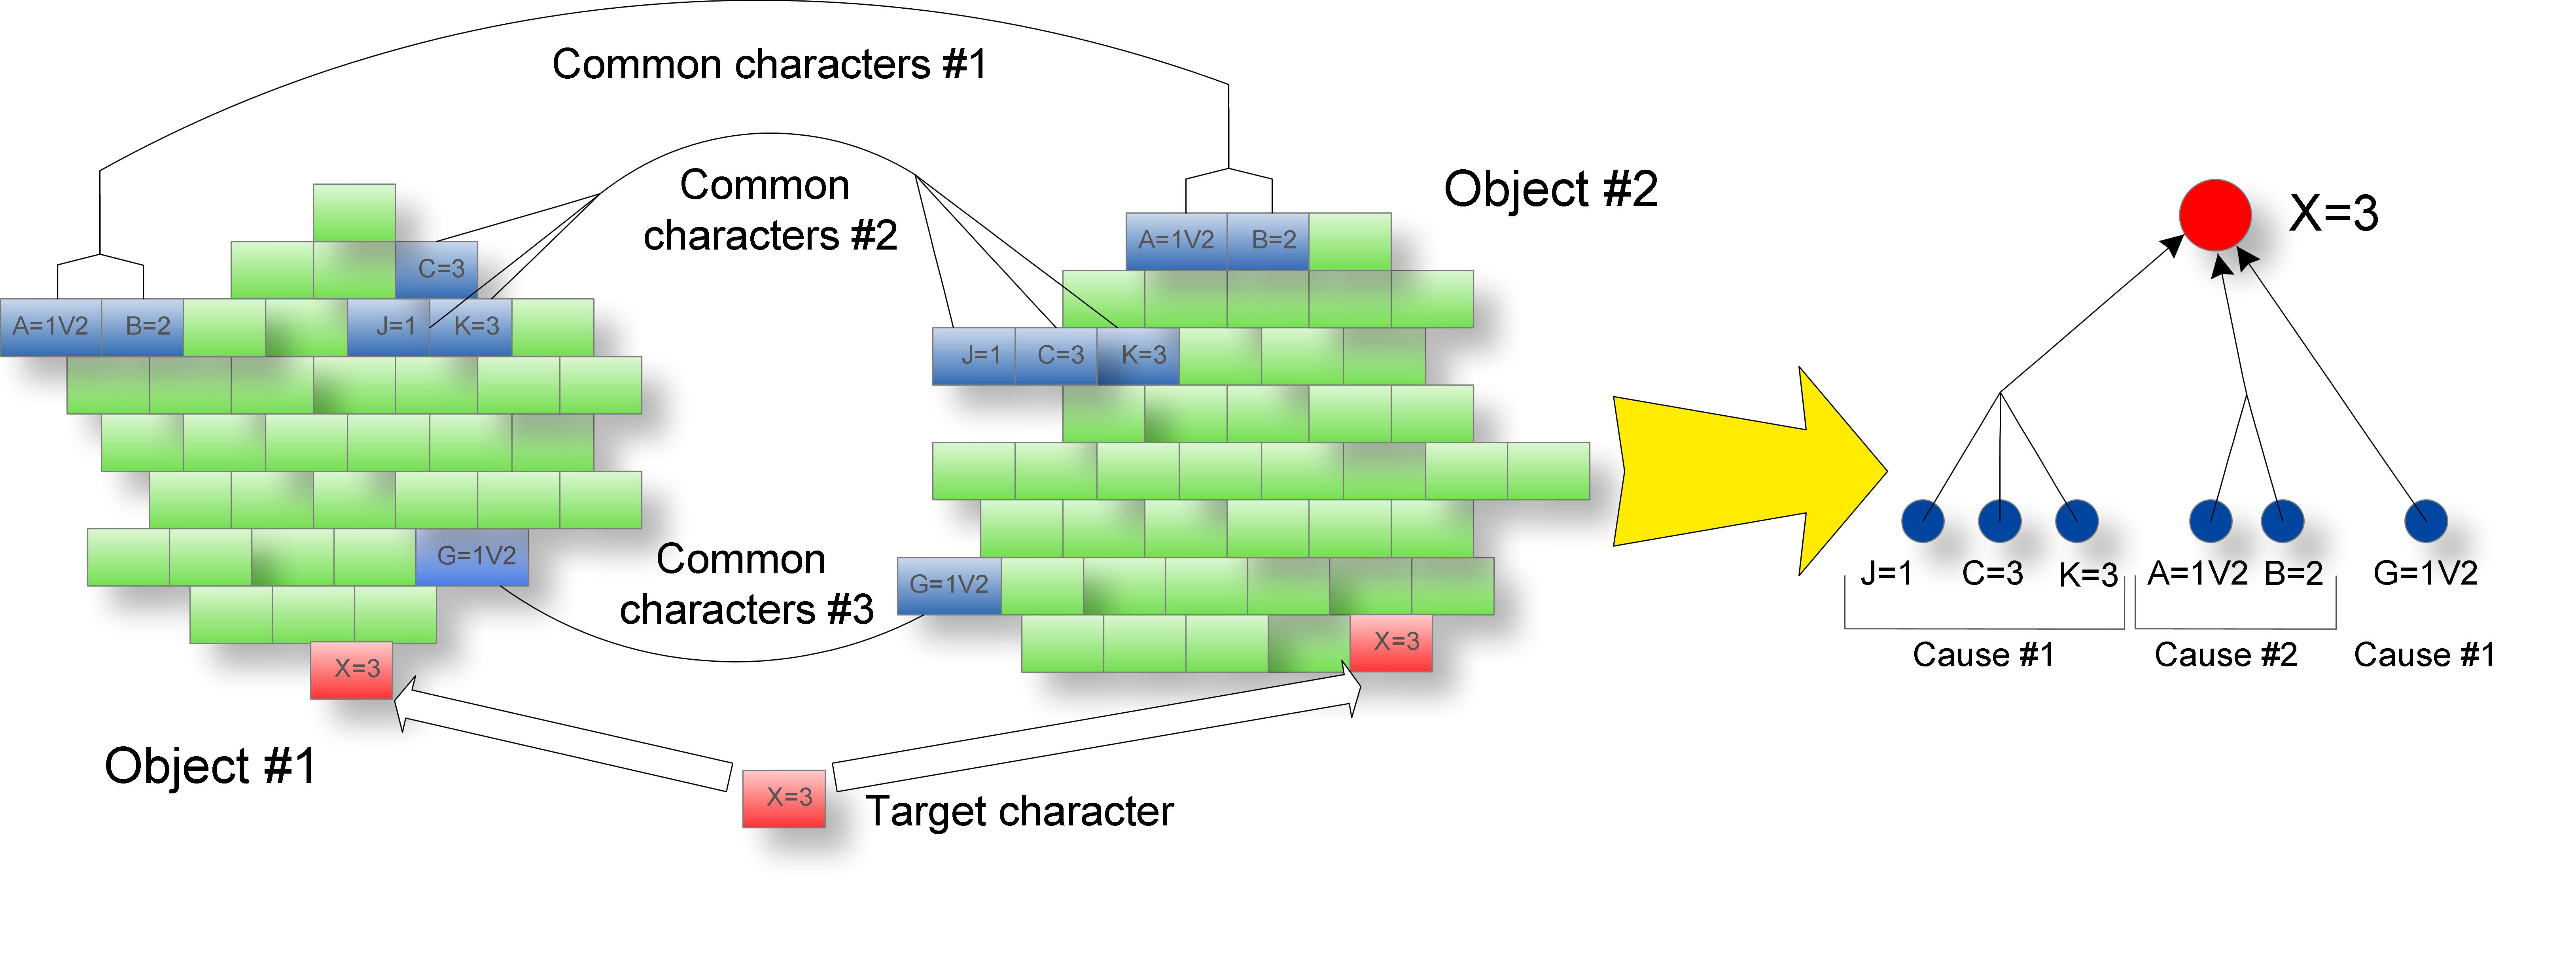
\includegraphics[width=\textwidth]{JSMProcess.jpeg}
	\end{frame}
	
	\begin{frame}
		\frametitle{Фальсификация гипотез}
		\scriptsize
		Алгоритм перевода ДСМ гипотез в диаграмму путей:
		\begin{itemize}
			\item Наблюдаемые переменные $X'=\{x_1,x_2,\dots,x_m\}$ "--- множество признаков $f_1, f_2,\dots, f_n$, участвующих в гипотезе, в том числе и целевая.
			\item Латентные переменные  "--- признаки из комплексных свойств причин $d^j$.
			\item Наличие интервалов учиытвается при определении параметров модели $a_1, a_2,\dots$.
			\item Запуск итерационного процедуры проверки соответствия дисперсий и ковариаций имеющимся данным.
		\end{itemize}
		\centering
		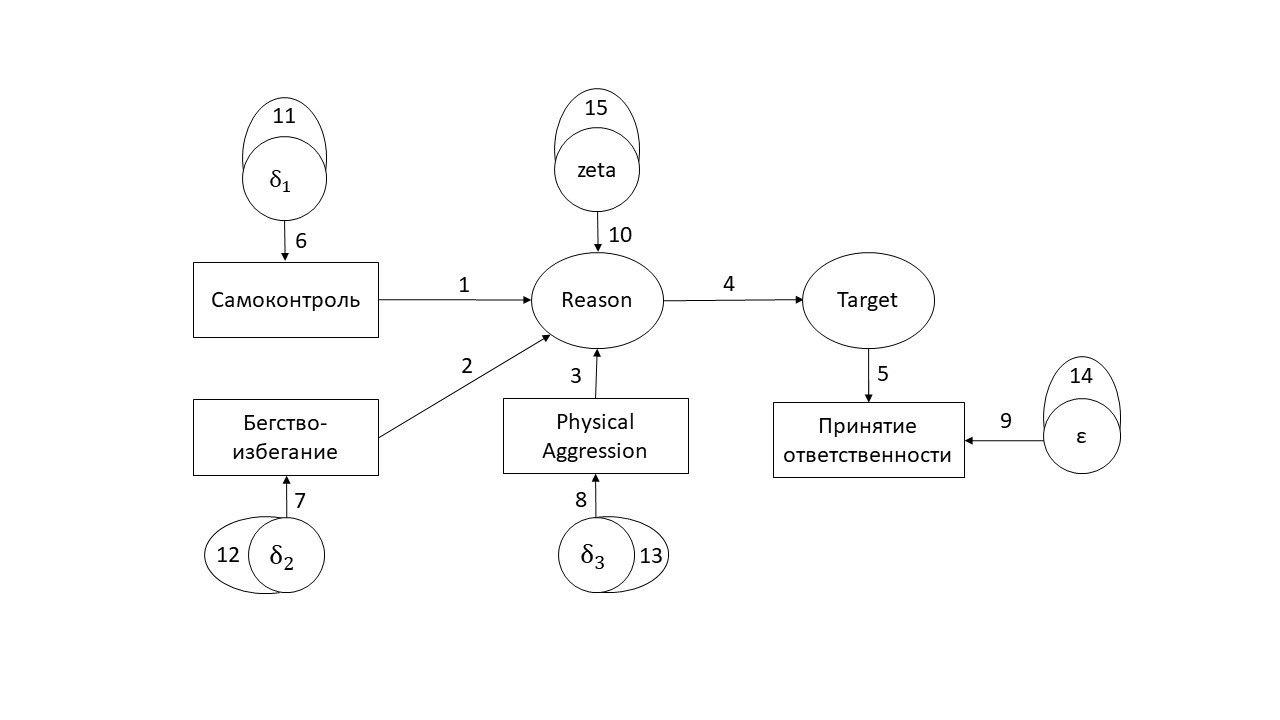
\includegraphics[width=0.7\textwidth]{hyp.jpg}
	\end{frame}
	
	\begin{frame}
		\frametitle{Список публикаций}
		
		\nocite{*}
		\printbibliography[resetnumbers=true]
	\end{frame}	
				
	\begin{frame}
		\centering
		\Huge
		Спасибо за внимание!
		\normalsize
		\par\bigskip
		\par\bigskip
		\par\bigskip
		pan@isa.ru
		\par\bigskip
		\url{https://github.com/cog-isa/aqjsm}
	\end{frame}			
\end{document}
	
	
